\chapter{Background}
\label{cha:background}
This chapter provides an overview of the text mining field along with previous work in the area and all necessary background information required to understand the major tasks involved in this project.

\section{Text Mining}
\label{sec:textmining}
``Text mining is the process of extracting interesting information and knowledge from unstructured text"\cite{hotho-etal-ldv-2005}.
\begin{figure}
\begin{center}
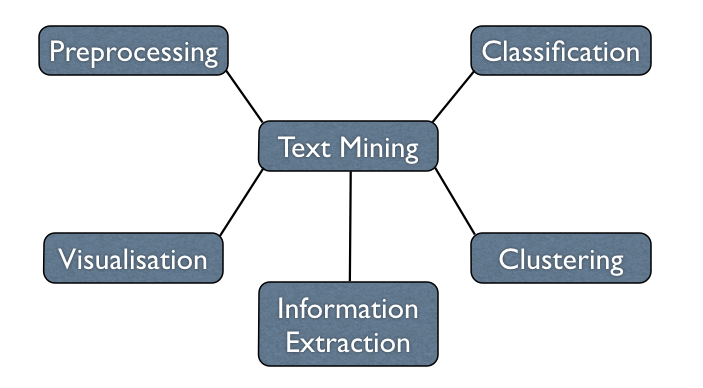
\includegraphics[width=10cm]{textmining}
\end{center}
\caption{Aspects of text mining}
\label{fig:design}  
\end{figure}

\section[Sentiment Analysis]{Sentiment Analysis and Opinion Mining}

\section{Twitter Mining}
There has been several previous works on text mining Twitter posts, however, the bulk of these have focussed solely on biomedicine and the financial sector.


% MOVE TWITTER API HERE? FROM IMPLEMENTATION CHAPTER